\documentclass[a4paper]{article}
\usepackage{fullpage}
\usepackage{amsmath}
\usepackage{amssymb}
\usepackage{tikz}
\usetikzlibrary{positioning}

\author{Angermueller Christof}
\date{10 January 2014}
\title{Bayesian variational inference for a mixture of factor analyzer}

\begin{document}
\maketitle

\newcommand{\bs}{\boldsymbol}
\newcommand{\Xy}{\bs{y}^{n,g}}
\newcommand{\Xx}{\bs{x}^n}
\newcommand{\Xz}{\bs{z}^n}
\newcommand{\XR}{\mathbb{R}}

\section{Model}
\subsection{Notations}
\begin{table}[h]
  \begin{center}
  \begin{tabular}{ll}
    $n=1,...,N$ & Samples \\
    $g=1,...,G$ & Genes \\
    $k=1,...,K$ & Factor analyzers \\
    $D$ & Number of observed variables \\
    $E$ & Number of latent variables \\
    $\Xy\in\XR^D$ & Counts sample $n$ gene $g$ \\
    $\Xx\in\XR^E$ & Factors sample $n$ \\
    $\Xz\in\{0,1\}^K$ & Indicator factor analyzers sample $n$ \\
    $\bs{\pi}\in\XR^K$ & Mixture coefficients \\
    $\Lambda^k\in\XR^{D\times E}$ & Precision matrix factor analyser $k$
  \end{tabular}
\end{center}
\end{table}

\begin{figure}[h]
  \begin{center}
    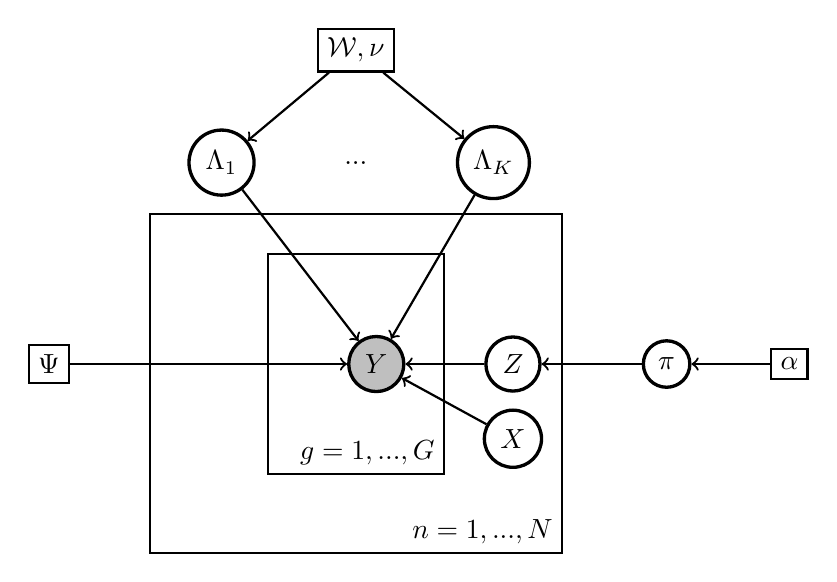
\begin{tikzpicture}
      \tikzstyle{sVar}=[circle, draw=black, very thick];
      \tikzstyle{sPlate}=[rectangle, draw=black, thick, align=flush right];
      \tikzstyle{sHyper}=[rectangle, draw=black, thick];
      \tikzstyle{sDep}=[->, thick];

      \node[sPlate, text width=5cm, text height=4cm] (Pn) {$n=1,...,N$};
      \node[sPlate, text width=2cm, text height=2.5cm, below=.5cm of Pn.north] (Pg) {$g=1,...,G$};
      \node[sVar, left=.5 of Pg.east, fill=gray!50] (Y) {$\bs{Y}$};
      \node[sVar, right=.5cm of Pg.east] (Z) {$\bs{Z}$};
      \node[sVar, below=.2cm of Z] (X) {$\bs{X}$};
      \node[sVar, right=2.5cm of Pg.east] (Pi) {$\bs{\pi}$};
      \node[sHyper, left=2.5cm of Pg.west] (Psi) {$\Psi$};
      \node[sHyper, right=1cm of Pi] (Alpha) {$\bs{\alpha}$};
      \node[above=.5 of Pn.north] (Dots) {...};
      \node[sVar, left=1cm of Dots] (Lambda1) {$\Lambda_1$};
      \node[sVar, right=1cm of Dots] (LambdaK) {$\Lambda_K$};
      \node[sHyper, above=1cm of Dots] (Wish) {$\mathcal{W},\nu$};
      \draw[sDep] (Z) -- (Y);
      \draw[sDep] (X) -- (Y);
      \draw[sDep] (Psi) -- (Y);
      \draw[sDep] (Pi) -- (Z);
      \draw[sDep] (Alpha) -- (Pi);
      \draw[sDep] (Lambda1) -- (Y);
      \draw[sDep] (LambdaK) -- (Y);
      \draw[sDep] (Wish) -- (Lambda1);
      \draw[sDep] (Wish) -- (LambdaK);

    \end{tikzpicture}
  \end{center}
\end{figure}

\subsection{Factors}
\begin{align}
  P(\Xy|x^n,z^n,\Lambda,\Psi)=\prod_k N(\Xy|(\Lambda^k)^{-1} \Xx,\Lambda^k{\Lambda^k}^{-1}+\Psi)
\end{align}
\begin{align}
  P(\Xx)=N(\Xx|0,I_{E})
\end{align}
\begin{align}
  P(\Xz|\pi)=Mult(\Xz|\pi)
\end{align}
\begin{align}
  P(\Lambda^k)=\mathcal{W}(\Lambda^k|W, \nu)
\end{align}
\begin{align}
  P(\bs{\pi}|\alpha)=Dir(\bs{\pi}|\bs{\alpha})
\end{align}

\subsection{Evidence}
\begin{align}
  \prod_{n,g}P(\Xy)&=\int_{\bs{\theta}}P(\bs{\theta})\prod_{n,g}P(\Xy|\bs{\theta}) \\
                   &=\int_{\bs{\pi}}Dir(\bs{\pi}|\bs{\alpha})\int_\Lambda\prod_k\mathcal{W}(\Lambda^k|W,\nu) \\
                   &\quad\prod_n\left[\sum_k P(z_k^n|\bs{\pi})\int_{\Xx}N(\Xy|(\Lambda^k)^{-1} \Xx,\Lambda^k{\Lambda^k}^{-1}+\Psi)\right]
\end{align}


\end{document}
